\newcount\draft\draft=0
\documentclass{sigplanconf}
\usepackage{listings}
\usepackage{relsize}
\usepackage{hyperref}
\usepackage{xxx}
\usepackage{amsmath}
\usepackage{xspace}
\usepackage{graphicx}
\usepackage{microtype}
\usepackage{mathpartir,amsmath,amsthm}
\usepackage{amssymb}
\usepackage{csquotes}
\usepackage{tikz}
\usepackage{booktabs}
\usepackage{array}
\usepackage{textpos}
\usepackage{flushend}

\edef\perfdata#1{}%
\ifstrequal{#1}{normtime-gpswalk-lowc}{19.4\%}{}%
\ifstrequal{#1}{normtime-gpswalk-noopt}{11.9\%}{}%
\ifstrequal{#1}{normtime-gpswalk-sample}{11.3\%}{}%
\ifstrequal{#1}{normtime-hotspot-dummy}{100.0\%}{}%
\ifstrequal{#1}{normtime-hotspot-lowc}{40.5\%}{}%
\ifstrequal{#1}{normtime-hotspot-noopt}{4.4\%}{}%
\ifstrequal{#1}{normtime-hotspot-sample}{7.8\%}{}%
\ifstrequal{#1}{normtime-inversek2j-dummy}{100.2\%}{}%
\ifstrequal{#1}{normtime-inversek2j-lowc}{17.3\%}{}%
\ifstrequal{#1}{normtime-inversek2j-noopt}{4.9\%}{}%
\ifstrequal{#1}{normtime-inversek2j-sample}{1.6\%}{}%
\ifstrequal{#1}{normtime-kmeans-dummy}{100.7\%}{}%
\ifstrequal{#1}{normtime-kmeans-lowc}{434.2\%}{}%
\ifstrequal{#1}{normtime-kmeans-noopt}{21.4\%}{}%
\ifstrequal{#1}{normtime-kmeans-sample}{18.0\%}{}%
\ifstrequal{#1}{normtime-salary-abs-dummy}{100.3\%}{}%
\ifstrequal{#1}{normtime-salary-abs-lowc}{733.1\%}{}%
\ifstrequal{#1}{normtime-salary-abs-noopt}{102.2\%}{}%
\ifstrequal{#1}{normtime-salary-abs-sample}{24.0\%}{}%
\ifstrequal{#1}{normtime-salary-dummy}{100.0\%}{}%
\ifstrequal{#1}{normtime-salary-lowc}{51.6\%}{}%
\ifstrequal{#1}{normtime-salary-noopt}{54.2\%}{}%
\ifstrequal{#1}{normtime-salary-sample}{1.7\%}{}%
\ifstrequal{#1}{normtime-sobel-dummy}{100.0\%}{}%
\ifstrequal{#1}{normtime-sobel-lowc}{223.5\%}{}%
\ifstrequal{#1}{normtime-sobel-noopt}{24.3\%}{}%
\ifstrequal{#1}{normtime-sobel-sample}{7.5\%}{}%
\ifstrequal{#1}{o-normtime-harmmean-dummy}{100.2\%}{}%
\ifstrequal{#1}{o-normtime-harmmean-lowc}{43.4\%}{}%
\ifstrequal{#1}{o-normtime-harmmean-noopt}{11.1\%}{}%
\ifstrequal{#1}{o-normtime-harmmean-sample}{4.2\%}{}%
\ifstrequal{#1}{o-normtime-max-dummy}{100.0\%}{}%
\ifstrequal{#1}{o-normtime-max-noopt}{102.2\%}{}%
\ifstrequal{#1}{o-normtime-max-sample}{24.0\%}{}%
\ifstrequal{#1}{o-normtime-min-dummy}{100.0\%}{}%
\ifstrequal{#1}{o-normtime-min-noopt}{4.4\%}{}%
\ifstrequal{#1}{o-normtime-min-sample}{1.6\%}{}%
\ifstrequal{#1}{o-speedup-harmmean-dummy}{1.0$\times$}{}%
\ifstrequal{#1}{o-speedup-harmmean-lowc}{2.3$\times$}{}%
\ifstrequal{#1}{o-speedup-harmmean-noopt}{9$\times$}{}%
\ifstrequal{#1}{o-speedup-harmmean-sample}{24$\times$}{}%
\ifstrequal{#1}{time-gpswalk-dummy-analyze}{$<0.1$}{}%
\ifstrequal{#1}{time-gpswalk-dummy-run}{$537.0$}{}%
\ifstrequal{#1}{time-gpswalk-dummy-total}{$537$}{}%
\ifstrequal{#1}{time-gpswalk-lowc-analyze}{$1.5$}{}%
\ifstrequal{#1}{time-gpswalk-lowc-run}{$2.0$}{}%
\ifstrequal{#1}{time-gpswalk-lowc-total}{$3.5$}{}%
\ifstrequal{#1}{time-gpswalk-noopt-analyze}{$1.4$}{}%
\ifstrequal{#1}{time-gpswalk-noopt-run}{$62$}{}%
\ifstrequal{#1}{time-gpswalk-noopt-total}{$63$}{}%
\ifstrequal{#1}{time-gpswalk-sample-analyze}{$1.6$}{}%
\ifstrequal{#1}{time-gpswalk-sample-run}{$59.0$}{}%
\ifstrequal{#1}{time-gpswalk-sample-total}{$60$}{}%
\ifstrequal{#1}{time-hotspot-dummy-analyze}{$<0.1$}{}%
\ifstrequal{#1}{time-hotspot-dummy-run}{$422.0$}{}%
\ifstrequal{#1}{time-hotspot-dummy-total}{$422$}{}%
\ifstrequal{#1}{time-hotspot-lowc-analyze}{$4.7$}{}%
\ifstrequal{#1}{time-hotspot-lowc-run}{$0.9$}{}%
\ifstrequal{#1}{time-hotspot-lowc-total}{$5.7$}{}%
\ifstrequal{#1}{time-hotspot-noopt-analyze}{$1.7$}{}%
\ifstrequal{#1}{time-hotspot-noopt-run}{$16$}{}%
\ifstrequal{#1}{time-hotspot-noopt-total}{$18$}{}%
\ifstrequal{#1}{time-hotspot-sample-analyze}{$4.7$}{}%
\ifstrequal{#1}{time-hotspot-sample-run}{$28.0$}{}%
\ifstrequal{#1}{time-hotspot-sample-total}{$33$}{}%
\ifstrequal{#1}{time-inversek2j-dummy-analyze}{$<0.1$}{}%
\ifstrequal{#1}{time-inversek2j-dummy-run}{$4.8$}{}%
\ifstrequal{#1}{time-inversek2j-dummy-total}{$4.8$}{}%
\ifstrequal{#1}{time-inversek2j-lowc-analyze}{$<0.1$}{}%
\ifstrequal{#1}{time-inversek2j-lowc-run}{$<0.1$}{}%
\ifstrequal{#1}{time-inversek2j-lowc-total}{$<0.1$}{}%
\ifstrequal{#1}{time-inversek2j-noopt-analyze}{$<0.1$}{}%
\ifstrequal{#1}{time-inversek2j-noopt-run}{$0.2$}{}%
\ifstrequal{#1}{time-inversek2j-noopt-total}{$0.2$}{}%
\ifstrequal{#1}{time-inversek2j-sample-analyze}{$<0.1$}{}%
\ifstrequal{#1}{time-inversek2j-sample-run}{$<0.1$}{}%
\ifstrequal{#1}{time-inversek2j-sample-total}{$<0.1$}{}%
\ifstrequal{#1}{time-kmeans-dummy-analyze}{$<0.1$}{}%
\ifstrequal{#1}{time-kmeans-dummy-run}{$1.8$}{}%
\ifstrequal{#1}{time-kmeans-dummy-total}{$1.9$}{}%
\ifstrequal{#1}{time-kmeans-lowc-analyze}{$0.3$}{}%
\ifstrequal{#1}{time-kmeans-lowc-run}{$<0.1$}{}%
\ifstrequal{#1}{time-kmeans-lowc-total}{$0.3$}{}%
\ifstrequal{#1}{time-kmeans-noopt-analyze}{$0.4$}{}%
\ifstrequal{#1}{time-kmeans-noopt-run}{$<0.1$}{}%
\ifstrequal{#1}{time-kmeans-noopt-total}{$0.4$}{}%
\ifstrequal{#1}{time-kmeans-sample-analyze}{$0.3$}{}%
\ifstrequal{#1}{time-kmeans-sample-run}{$<0.1$}{}%
\ifstrequal{#1}{time-kmeans-sample-total}{$0.3$}{}%
\ifstrequal{#1}{time-salary-abs-dummy-analyze}{$0.2$}{}%
\ifstrequal{#1}{time-salary-abs-dummy-run}{$87.0$}{}%
\ifstrequal{#1}{time-salary-abs-dummy-total}{$87$}{}%
\ifstrequal{#1}{time-salary-abs-lowc-analyze}{$21$}{}%
\ifstrequal{#1}{time-salary-abs-lowc-run}{$0.2$}{}%
\ifstrequal{#1}{time-salary-abs-lowc-total}{$21$}{}%
\ifstrequal{#1}{time-salary-abs-noopt-analyze}{$0.4$}{}%
\ifstrequal{#1}{time-salary-abs-noopt-run}{$89$}{}%
\ifstrequal{#1}{time-salary-abs-noopt-total}{$89$}{}%
\ifstrequal{#1}{time-salary-abs-sample-analyze}{$20.0$}{}%
\ifstrequal{#1}{time-salary-abs-sample-run}{$0.2$}{}%
\ifstrequal{#1}{time-salary-abs-sample-total}{$21$}{}%
\ifstrequal{#1}{time-salary-dummy-analyze}{$<0.1$}{}%
\ifstrequal{#1}{time-salary-dummy-run}{$150.0$}{}%
\ifstrequal{#1}{time-salary-dummy-total}{$150$}{}%
\ifstrequal{#1}{time-salary-lowc-analyze}{$2.6$}{}%
\ifstrequal{#1}{time-salary-lowc-run}{$<0.1$}{}%
\ifstrequal{#1}{time-salary-lowc-total}{$2.6$}{}%
\ifstrequal{#1}{time-salary-noopt-analyze}{$0.2$}{}%
\ifstrequal{#1}{time-salary-noopt-run}{$81$}{}%
\ifstrequal{#1}{time-salary-noopt-total}{$81$}{}%
\ifstrequal{#1}{time-salary-sample-analyze}{$2.5$}{}%
\ifstrequal{#1}{time-salary-sample-run}{$<0.1$}{}%
\ifstrequal{#1}{time-salary-sample-total}{$2.6$}{}%
\ifstrequal{#1}{time-sobel-dummy-analyze}{$<0.1$}{}%
\ifstrequal{#1}{time-sobel-dummy-run}{$37.0$}{}%
\ifstrequal{#1}{time-sobel-dummy-total}{$37$}{}%
\ifstrequal{#1}{time-sobel-lowc-analyze}{$2.8$}{}%
\ifstrequal{#1}{time-sobel-lowc-run}{$<0.1$}{}%
\ifstrequal{#1}{time-sobel-lowc-total}{$2.8$}{}%
\ifstrequal{#1}{time-sobel-noopt-analyze}{$2.2$}{}%
\ifstrequal{#1}{time-sobel-noopt-run}{$6.9$}{}%
\ifstrequal{#1}{time-sobel-noopt-total}{$9.1$}{}%
\ifstrequal{#1}{time-sobel-sample-analyze}{$2.8$}{}%
\ifstrequal{#1}{time-sobel-sample-run}{$<0.1$}{}%
\ifstrequal{#1}{time-sobel-sample-total}{$2.8$}{}%
}


\lstset{%
    language=Java,
    emph={@Approx, @Precise, @Top, @Context, endorse, @Approximable, assert,
    passert},
    emphstyle=\bfseries,
    columns=fullflexible,
    basicstyle=\sffamily\small,
    aboveskip=1mm plus 1mm minus 1mm,
    belowskip=1mm plus 1mm minus 1mm,
    mathescape=true,
}

\hypersetup{%
    colorlinks=false,
    hidelinks
}

% Tolerate quotes like "this" instead of like ``this''.
\MakeOuterQuote{"}

% Math macros for probability stuff.
\newcommand{\prob}[1]{\ensuremath{\Pr\!\left[#1\right]}}
\newcommand{\expc}[1]{\ensuremath{\mathrm{E}\!\left[#1\right]}}
\newcommand{\varc}[1]{\ensuremath{\mathrm{Var}\!\left[#1\right]}}
\newcommand{\code}[1]{\lstinline[language=Python]{#1}}

\providecommand{\unct}[1]{\ensuremath{\mathit{Uncertain}\langle \mathit{#1} \rangle}\xspace}

% Text macros.
\newcommand{\lil}{\lstinline}
\newcommand{\passert}{\textsf{passert}\xspace}
\newcommand{\passerts}{\textsf{passert}s\xspace}
\newcommand{\Passert}{\textsf{Passert}\xspace}
\newcommand{\Passerts}{\textsf{Passert}s\xspace}
\newcommand{\tool}{\textsc{Mayhap}\xspace} % feel free to come up with a better name!
\newcommand{\mayhap}{\textsc{Mayhap}\xspace} % feel free to come up with a better name!
\newcommand{\lang}{\textsc{Prob}\xspace} % feel free to come up with a better name!
\newcommand{\corelang}{\textsc{ProbCore}\xspace} % me too!
\newcommand{\bench}[1]{\textsf{#1}}
                                

% For the semantics.
\newcommand{\defeq}{\equiv}
\newcommand{\judge}{\Downarrow}
\newcommand{\alt}{\:|\:}
\newtheorem{theorem}{Theorem}

\usepackage{comment}

\newcommand{\fix}[2]{{\bf #1 asks:~\emph{#2}}}

% Show Mercurial revision number.
\ifnum\draft=1
  \InputIfFileExists{revision}{}{\newcommand{\Revision}{?}}
  \usepackage{drafthead}
\fi

\begin{document}

\title{Expressing and Verifying Probabilistic Assertions}
\authorinfo{Adrian Sampson ~~ Pavel Panchekha}{University of Washington}{}
\authorinfo{Todd Mytkowicz ~~ Kathryn S. McKinley}{Microsoft Research}{}
\authorinfo{Dan Grossman ~~ Luis Ceze}{University of Washington}{}

% sigplanconf stuff
\conferenceinfo{PLDI '14}{June 9--11 2014, Edinburgh, United Kingdom}
\copyrightyear{2014}
\copyrightdata{978-1-4503-2784-8/14/06}
\doi{2594291.2594294}
\titlebanner{}
\preprintfooter{}

\maketitle

\abstract{%
  % toddm: inference as example for ML

  Traditional assertions express correctness properties that must hold
  on every program execution.  However, many applications have
  probabilistic outcomes and consequently their correctness properties
  are also probabilistic (e.g., they identify faces in images, consume
  sensor data, or run on unreliable hardware). Traditional
  assertions do not capture these correctness
  properties. % and current verification tools prove
  % properties that hold for \emph{every} execution
  % For programs with
  % probabilistic outcomes, we
  This paper proposes that programmers express probabilistic
  correctness properties with \emph{probabilistic assertions} and
  describes a new \emph{probabilistic evaluation} approach to
  efficiently verify these assertions.
 %  To which this paper proposes \emph{probabilistic assertions} and
 %  \emph{probabilistic evaluation}. % to efficiently verify them.
  Probabilistic assertions are Boolean expressions that express the
  \emph{probability} that a property will be true in a given execution
  rather than asserting that the property must always be true.
  Given either specific inputs or distributions on the input space,
  probabilistic evaluation verifies probabilistic assertions
  by first performing \emph{distribution
    extraction} to represent the program
  as a Bayesian network. Probabilistic evaluation then uses statistical
  properties to simplify
  this representation to efficiently compute assertion
  probabilities directly or with sampling.  Our approach is a mix of
  both static and dynamic analysis: distribution extraction
  statically
  builds and optimizes the Bayesian network representation and
  sampling dynamically interprets this representation.
  We implement our approach in a
  tool called \tool for C and C++ programs. We evaluate
  expressiveness, correctness, and performance of \tool on programs
  that use sensors, perform approximate computation, and obfuscate
  data for privacy.  Our case studies demonstrate that probabilistic
  assertions describe useful correctness properties and that \tool
  efficiently verifies them.

  % We evaluate an implementation of the analysis using C and C++ programs
  % that use sensors, perform approximate computation, and obfuscate
  % data for privacy.
  % We demonstrate that probabilistic assertions express useful properties of
  % these programs that are not captured by traditional assertions. 
  % And, our analysis evaluates probabilistic assertions \xxx{?} faster on average
  % than a naive checker.
}

%%% Local Variables: 
%%% mode: latex
%%% TeX-master: "paper"
%%% End: 


% \category{F.1.2}{Computation by Abstract Devices}{Modes of Computation---Probabilistic computation}
\category{G.3}{Probability and Statistics}{Statistical computing}
\category{D.2.5}{Software Engineering}{Testing and Debugging---Symbolic execution}
%
% AEC "Artifact Evaluated" badge.
\begin{tikzpicture}[remember picture,overlay]
    \node [shift={(-0.9in,-0.9in)}]  at (current page.north east) {
        \includegraphics[scale=0.1]{aec-badge-pldi.pdf}
    };
\end{tikzpicture}
%
\terms
Languages, Reliability

\keywords
Probabilistic programming,
approximate computing,
data obfuscation,
differential privacy,
sensors,
symbolic execution

\section{Introduction}
Traditional assertions express logical properties that help programmers design and
reason about the correctness of their program. Verification tools
guarantee that every execution will satisfy an assertion, such as the
absence of null dereferences or a legal value range for a variable.
However, many applications produce or consume probabilistic data, such as the
relevance of a document to a search, the distance to the nearest
coffee shop,
or the estimated arrival time of the next bus. From smartphones with
sensors to robots to machine learning to big data to approximate
computation, many applications compute with probabilistic
values.  % Programming with unreliable hardware also involves
% probabilistic computation~\cite{rely, enerj, npu}.

Current assertion languages and verification tools are insufficient in
this domain.  Traditional assertions do not capture probabilistic
correctness because they demand that a property hold on \emph{every}
execution.  Recent work on inference in probabilistic programming
languages builds language abstractions to aid programmers in describing
machine learning models but
does not deal with verification of probabilistic correctness
properties~\cite{infernet, church, pmonad, PPT:05}. Sankaranarayanan et al.~\cite{sriram-pldi} address the
verification of programs in probabilistic programming
languages through polyhedral volume estimation,
but this approach limits the domain to programs with linear arithmetic
over constrained probability distributions.
In contrast, this paper
builds on Bornholt et al.'s \unct{T}~\cite{uncertaint},
which defines a semantics for computing in mainstream languages over a broader set of distributions
with sampling functions
but does not verify programs.

This paper proposes \emph{probabilistic assertions}
(\passerts), which express probabilistic program properties, and
\emph{probabilistic evaluation}, which verifies them.  A \passert
statement is a probabilistic logical statement over random
variables. \emph{Probabilistic evaluation} extracts, optimizes, and
evaluates the distribution specified in a \passert by
combining techniques from static verification,
symbolic execution, and dynamic testing.

\paragraph*{Probabilistic Assertions} 
Programmers write \code{passert e, p, cf}
to check the probability that the Boolean expression \code{e} holds in
a given execution of the program is at least \code{p} with confidence
\code{cf}. The parameters \code{p} (defaults to 0.5) and \code{cf}
(defaults to 95\%) are optional. Our analysis estimates the likelihood
that \code{e} is true, bounds any error in that estimate, and determines
whether that
estimate is significantly different from
\code{p}. 
For example, consider the following function, which adds
Gaussian noise to users' true locations to protect their privacy.
%
\begin{lstlisting}
  def obfuscate_location(location):
    noise = random.gauss(0,1)
    d = distance(location, location + noise)
    passert d < 10, 0.9, 95%
    return location + noise
\end{lstlisting}
%
To ensure that obfuscation does not change a user's true location too
much, the programmer asserts that the Euclidean distance between the
true and obfuscated location should be within 10 miles at least 90\%
of the time with 95\% confidence. While occasional outliers are
acceptable, the programmer wants to ensure that the common case is
sufficiently accurate and therefore useful.

A traditional assertion---\code{assert d < 10}---does not
express this intent.  Since the Gaussian distribution has a non-zero
chance of adding any amount of noise, some executions will make
\code{d} greater than 10.  Since these infrequent outlier cases are possible,
traditional verification must conclude that the assertion does not hold.

\paragraph*{Probabilistic Evaluation} Probabilistic evaluation
verifies the probabilistic logical statement over random variables
expressed by the \passert. It first performs \emph{distribution extraction},
which is a symbolic execution that builds a Bayesian
network, a directed, acyclic graphical model. Nodes
represent random variables from the program and edges between nodes
represent conditional dependences between those random variables.
This process defines a probabilistic semantics in which \emph{all}
variables are distributions. Constants (e.g., \code{x = 3}) are
point-mass distributions.  Random distributions, both simple (uniform,
Gaussian, etc.) and programmer-defined, are represented
symbolically.  Other variables are defined in terms of these basic
distributions.

For example, let $L$,
$D$, and $N$ be the random variables corresponding to the variables
\code{location}, \code{d}, and \code{noise} in the above program.  The
\passert constrains the probability $\prob{D < 10}$ given that $L$ is
a point-mass distribution and that $N$ is drawn from a Gaussian:
%
$$ \prob{D < 10~|~L = \mathsf{location}, N \sim \mathcal{N}(0,1)} > 0.9 $$
%
This inequality constrains the probability of correctness for a particular
input location.  Alternatively, programmers may express a distribution
over expected input locations by, for example, setting the
\code{location} variable to sample from a uniform distribution. The
\passert then measures the likelihood that the obfuscation will yield
acceptable results for uniformly distributed input locations:
%
$$ \prob{D < 10~|~L \sim \mathcal{U}, N \sim \mathcal{N}(0,1)} > 0.9 $$

\begin{figure}
    \begin{center}
    \includegraphics[width=\columnwidth]{figs/overview.pdf}
    \end{center}
    \vspace*{-1.0ex}
    \caption{\tool's workflow to verify probabilistic
    assertions.}
    \label{passert:fig:overview}
\end{figure}


Our key insight is that, with this probabilistic semantics for
\passerts, we can optimize the Bayesian network representation and
significantly improve the efficiency of verification.  Using known
statistical properties, our optimizations produce a simplified but
equivalent Bayesian network. For example, we exploit identities of
common probability distributions and Chebyshev's inequality.  In some
cases, these simplifications are sufficient to facilitate direct
computation and verify the \passert precisely. Otherwise, we sample
the simplified Bayesian network and perform a hypothesis test to
statistically verify the \passert. We use
\emph{acceptance sampling}, a form of hypothesis testing, to bound the
chance of both false positives and false negatives subject to a
confidence level.  Programmers can adjust the confidence level to
trade off between analysis time and verification accuracy.


\paragraph*{Evaluation}
We implement this approach in a tool called \tool that takes C and C++
programs with \passerts as inputs. \tool emits either \emph{true},
\emph{false}, or \emph{unverifiable} along with a confidence interval
on the assertion's probability.  Figure~\ref{passert:fig:overview} gives an
overview.  We implement the entire toolchain for \tool in the LLVM
compiler infrastructure~\cite{llvm}.  First, \tool transforms a
probabilistic C/C++ program into a Bayesian network that expresses the
program's probabilistic semantics. For program inputs, developers
provide concrete values or describe input distributions. \tool
optimizes the Bayesian-network
representation using statistical properties and then either
evaluates the network directly or performs sampling.

We implement case
studies from three application domains: sensors, data obfuscation, and
approximate computing.  We show that \passerts express their
correctness properties and that \mayhap offers an average speedup of
\perfdata{o-speedup-harmmean-sample} over stress testing with rote
sampling.
\tool's benefits over simple stress testing---repeated execution of
the original program---are threefold. First, statistical
simplifications to the Bayesian network representation reduce the work
required to compute each sample:
for example, reducing the sum of two
Gaussian distributions into a single Gaussian halves the necessary
number of samples.
Second, distribution extraction has the effect of
partially evaluating the probabilistic program to slice away the
non-probabilistic parts of the computation. Sampling the resulting
Bayesian network eliminates wasteful re-execution of deterministic
code. Third, our approach either directly evaluates the \passert or derives
a number of samples sufficient for statistical significance.
It thereby provides statistical guarantees
on the results of sampling that blind stress testing does not guarantee.

Although programs that compute with probabilistic data are already
ubiquitous, abstractions and tools to help their developers are
lagging.  By harnessing randomness, our approach introduces new and
effective abstractions for correctness, optimization, and
verification of probabilistic programs.

%%% Local Variables: 
%%% mode: latex
%%% TeX-master: "paper"
%%% End: 

\section{Programming Model}
\label{sec:model}
 
This section presents an intuitive view of programs as probabilistic
computations over random variables.
For our purposes, a probabilistic program is an ordinary imperative program
that calls sampling functions for probability distributions~\cite{kozen}.
Consider this simple program:
%
\begin{lstlisting}
  x = random.uniform(0,1)
  w = 0.9
  passert x < w, 0.90
\end{lstlisting}
%
This program samples from a uniform distribution, ranging from 0 to 1,
assigns a concrete value to \code{w}, and then asserts that the sample is
less than 0.9 using the comparison \code{x < w} with 90\% probability.
An invocation
of \code{random.uniform} returns one sample from the distribution.
The language provides a library of sampling functions for common distributions, such as uniform, Gaussian,
and Bernoulli distributions. Programmers may define sampling functions for new distributions using
arbitrary code.

Programmers write specifications of correctness in \passerts. The above \passert is
satisfied because the probability that a random sample from 
$\mathcal{U}(0,1)$ is less than 0.9 is exactly 90\%.

To formalize this reasoning, we represent programs as Bayesian networks.
A Bayesian network is
a directed, acyclic graphical model wherein nodes represent random variables and
edges represent conditional dependence between those
random variables.
%
\begin{center}
{\scriptsize
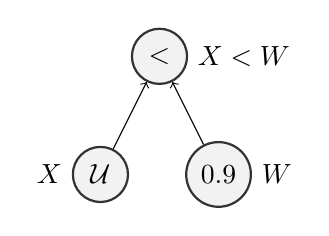
\begin{tikzpicture}[<-]
  \tikzstyle{op}=[circle, minimum size = 7mm, thick, draw =black!80, node distance = 5mm, fill=black!5]

  \node [op,label=right:$X < W$] {$<$}
    child{node [op,label=left:$X$] {$\mathcal{U}$}}
    child{node [op,label=right:$W$] {$0.9$}}
  ;
\end{tikzpicture}
}
\end{center}
%
Much like an expression tree, each node in the Bayesian network corresponds to a value produced by the program.  Unlike an expression tree, however, each node represents a distribution rather than a single value.
This network, for example,
contains three random variables ($X$, $W$, and $X<W$), one for each
expression executed in the program (\code{random.uniform(0,1)}, \code{0.9},
and \code{x < w}). The directed edges represent how these
random variables conditionally depend on one another. For example,
the node for the random variable $X
< W$ has edges from two other nodes: $X$ and $W$.

Because each variable is
dependent \emph{only} on its parents in a Bayesian network, the probability
distributions for each node are defined locally. In our example, the
distribution for the $X < W$ node, a Bernoulli random variable, is:
%
$$\prob{X<W~|~X \sim \mathcal{U}, W=0.9}$$
%
Computing the distribution for $X < W$ requires only the
distributions for its
parents, $X$ and $W$. In this case, both parents are leaves in the Bayesian
network: a uniform distribution and a point-mass distribution.

One way to compute the distribution is to sample it. Sampling the root node
consists of generating a sample at each leaf and then propagating the values
through the graph.
% A sample for any node can be computed based only on the samples of its
% parents.
Since Bayesian networks are acyclic, every node generates
only a single value per sample and the running time of each sample is
bounded.

In this example, we can exploit the Bayesian network formulation
to simplify the graph and compute an exact solution without
sampling. By definition, when $X$ is uniformly distributed,
for any constant $c \in [0,1]$, $\prob{X < c} = c$.  Using this
statistical knowledge, we replace the tree in our example with a
single node representing a Bernoulli distribution with probability
0.9.

% In our example, this optimization collapses the program's entire
% network to a single node. To test the \passert, we know exactly
% $\prob{X < W} = 0.9$, so the assertion succeeds and there is no need
% to sample. In general, more complex programs result in more complex
% Bayesian networks, which even after simplification, will require
% sampling.

% When sampling, we verify \passerts probabilistically with a bounded
% probability of error. A lower error probability generally means higher
% confidence in the verification but more cost to compute. We use
% hypothesis testing to verify a \passert probabilistically based on
% samples.  A hypothesis test requires three parameters: $B$,  a
% Bernoulli distribution to test (i.e., $X < W$); $\alpha$, the
% confidence level; and $u$, such that $\expc{B} >
% u$ at the $\alpha$ confidence level.  The programmer must provide the
% boolean expression to test, which induces $B$, but may use default
% parameters for $\alpha$ and $u$: 0.05 for $\alpha$ and 0.5 for
% $u$, which specifies that $B$ is more
% likely to be true than false with 95\% confidence.  Using a hypothesis
% test bounds the probabilities of both false positives and false
% negatives.  In cases where the necessary number of samples to meet the
% confidence levels is infeasible, the test returns an ``unknown''
% result, meaning that the \passert is neither proven nor disproven.
% Section~\ref{sec:sample} describes the hypothesis testing approach in
% more detail.

% Our verification
% implies that if we ran a program 100 times, we would say \code{B >
%   0.5} when in reality \code{B <= 0.5} at most 5\% of the time.  In
% other words, the confidence interval bounds false-positives.  To bound
% false-negatives, we use an over-approximation of the maximum variance
% in a Bernoulli distribution.


%\paragraph{Summary}
The Bayesian network abstraction for probabilistic programs yields two major
advantages.
First, it gives a probabilistic semantics to programs and \passert
statements.
Section~\ref{sec:semantics} formalizes our probabilistic semantics and proves that
sampling the Bayesian representation is equivalent to sampling the original
program.
Second, we exploit 
probabilistic algebras and statistical properties of random variables to optimize the
verification process. In some cases, we verify \passerts without sampling.
Section~\ref{sec:optim} introduces these 
optimizations.
% Third, we symbolically represent some loops that perform reductions over
% random variables as nodes in our Bayesian network, making them amenable to
% optimizations.  For all other loops, we use sampling to estimate their
% effect. 
% Section~\ref{sec:sample} discusses how we sample loops to probabilistically verify  \passerts and bound
% error in that verification.
% Removing this advantage since it seems unrelated to the Bayesian-network
% formulation. -ALDS



\section{Distribution Extraction} 
\label{sec:distex}


Given a program with a \passert $e$ and either a concrete input or a
distribution over inputs,
\tool performs a probabilistic evaluation
by building and optimizing a Bayesian-network representation of the statements
required to evaluate the \passert.  This section describes
distribution extraction, which is the first step in this process.
Distribution extraction produces a symbolic Bayesian network representation
that corresponds to the slice of the program contributing to $e$.
\tool treats randomness as symbolic and
deterministic components as concrete.
The process is similar to symbolic execution and to lazy evaluation in
functional languages.

\paragraph{Distributions as Symbolic Values}
\mayhap performs a forward pass over the program, concretely
evaluating deterministic computations and introducing symbolic
values---probability-distribution expression trees---to represent
probabilistic values. For example, the following statement: 
%
\begin{lstlisting}[language=Python]
  a = b + 2
\end{lstlisting}
%
computes $a$ concretely when $b$ is not probabilistic.  If, prior to the above
statement, the program assigns \lil{b = 5}, then we perform the
addition and set $a=7$.  However, if \lil{b = gaussian()}, we
add a node to the Bayesian network, representing $b$
symbolically as a Gaussian distribution.  We then create a sum node for
$a$ with two parents: $b$'s Gaussian  and $2$'s constant (point mass) distribution.

As this mixed symbolic and concrete execution proceeds, it eagerly
evaluates any purely deterministic statements but builds a Bayesian-network
representation
of the forward slice of any probabilistic statements.  This
process embodies a symbolic execution in which the symbolic values are
probability distributions. Our approach differs from typical symbolic
execution
in how it handles control flow (see below).  

When the analysis reaches a statement \passert $e$, \mayhap records the Bayesian network
rooted at $e$. It then optimizes the network and samples the
resulting distribution.
Compared to sampling the entire program repeatedly, sampling the extracted
distribution can be more efficient even without optimizations since it
eliminates redundant, non-probabilistic
computation. 

%  the work
% that would be wasted in a straightforward sampling approach to
% evaluating \passerts---by sampling the specialized distribution (as in
% Section~\ref{sec:sample}), we sample only the portion of the program
% that changes from execution to execution.

\label{sec:conditionals}


\paragraph{Conditionals}
% Any symbolic execution technique must address the possibility of control flow
% based on symbolic values. 
When conditionals and loops are based on purely
concrete values, distribution extraction proceeds down one side
of the control flow branch as usual. When conditions operate on probabilistic variables, the analysis
must capture the effect of both branch directions.

To analyze the probability distribution of a conditional statement,
we produce conditional probabilities
based on control-flow divergence. For example, consider this simple
program:
%
\begin{lstlisting}[language=Python]
  if a:  b = c   else:  b = d
\end{lstlisting}
%
in which $a$ is probabilistic. Even if both $c$
and $d$ are discrete, the value of $b$ is probabilistic since it depends on
the value of $a$. We can write the conditional probability distributions $\prob{B}$
for $b$ conditioned on both possible values for $a$:
%
\begin{align*}
  \Pr[B \;|\; A = \mathrm{true}] &= \Pr[C]\\
  \Pr[B \;|\; A = \mathrm{false}] &= \Pr[D]
\end{align*}
%
Instead, to simplify the representation of probabilities and to enable more
straightforward analysis, we \emph{marginalize} the condition $a$ to
produce an unconditional distribution for $b$. Using marginalization, we
write the unconditional distribution $\prob{B}$ as:
%
\begin{align*}
    \Pr[B] &= \sum_a \Pr[B\;|\; A = a] \prob{A = a} \\
           &= \Pr[B \;|\; A = \mathrm{true}] \prob{A = \mathrm{true}} \\
           & \qquad {}
            + \Pr[B \;|\; A = \mathrm{false}] \prob{A = \mathrm{false}} \\
           &= \Pr[C] \cdot \prob{A=\mathrm{true}} \\
           & \qquad {}
            + \Pr[D] \cdot (1 - \prob{A=\mathrm{true}})
\end{align*}
%
This expression computes the distribution for $b$ as a function of the
distributions for $a$, $c$, and $d$. Intuitively, the probabilistic evaluation rewrites
the condition to read \lil{b = a * c + (1 - a) * d}. This algebraic
representation enables some optimizations described
in Section~\ref{sec:expectation}.

\label{sec:loops}


\paragraph{Loops and External Code}
Loops with probabilistic conditions can, in general, run for an
unbounded number of iterations. Representing unbounded execution would
induce cycles in our graphical
model and violate the acyclic definition of a Bayesian network. For
example, consider a loop that accumulates samples and exits when the
sum reaches a threshold:
%
\begin{lstlisting}[language=Python]
  v = 0.0
  while v < 10.0:
    v += random.uniform(-0.5, 1.0)
\end{lstlisting}
%
If the random sample is negative in every iteration, then the
loop will never exit. The probability of this divergence is small but non-zero.

Prior work has dealt with probabilistic loops by restricting the program
to linear operators~\cite{sriram-pldi}. \tool relaxes this
assumption by treating a loop as a
black box that generates samples (i.e., the loop may run for an
unbounded but finite number of iterations), similar to a known
probability distribution such as \code{random.uniform}.
This representation avoids creating cycles.
In particular, \tool represents a loop body with a
\emph{summary node}, where variables read by the loop are
edges \emph{into} the node and variables written by the loop are edges \emph{out} of the node.

In practice, many loops in probabilistic programs have
non-probabilistic bounds. For example, we evaluated an image filter
(\bench{sobel}) that loops over the pixel array and applies a probabilistic
convolution to each window. The nested loops resemble:
%
\begin{lstlisting}[language=Python]
  for x in 0..width:
    for y in 0..height:
      filter(image[x][y])
\end{lstlisting}
%
While the computed pixel array contains probabilistic data, the dimensions
\code{width} and \code{height} are fixed
for a particular image. \tool extracts complete distributions from these common
concrete-bounded loops without black-box sampling.

\tool uses a similar black-box mechanism when interfacing with library code whose
implementation is not available for analysis---for example, when passing a
probabilistic value to the \code{cos()} function from the C standard library.
This straightforward approach prevents statistical optimizations inside the
library function or loop body but lets \tool analyze more programs.

\paragraph{Analyzing Loops with Probabilistic Path Pruning}
We propose another way to analyze loops with probabilistic bounds by
building on the path pruning techniques used in traditional symbolic
execution.  Typically, path pruning works by proving that some paths
are infeasible. If the analysis determines that a path constraint
is unsatisfiable, it halts exploration of that path.  Probabilistic evaluation
instead needs to discover when a given path is \emph{unlikely} rather
than impossible, i.e., when the conditions that lead to following this
path at run time have a probability that falls below a
threshold.  We propose tracking a path probability expression for each
explored path and periodically sampling these distributions to
prune unlikely paths.
This extension handles general probabilistic
control flow in programs that are likely to terminate eventually.
Intuitively, the more iterations the loop
executes, the less likely it is to execute another iteration.
Programs with a significant probability of running forever before
reaching a \passert can still prevent the analysis from terminating,
but this behavior likely indicates a bug.
We leave the evaluation of
this more precise analysis to future work.

% Assume a simple probabilistic program with a loop that lacks
% concrete bounds (i.e., the bounds are statistical).

% x = uniform(0,1)
% w = 0
% Label:
%   w += x + 1
%   if w < 100 goto Label
% z = w * 10
% passert z < 10

% Note we cannot naively represent this program as a Bayesian
% network because the loop induces a cycle in the induced graphical
% model.

% However, if we wrap the body of the loop into its own super-node
% we can remove the cycle in the graphical model and turn it into a
% Bayesian network---variables read within the body of the loop
% will be edges \emph{into} the super-node and variables written by
% the body of the loop will be edges \emph{out} of the super-node.
% This provides a mechanism to handle loops.  Of course, \tool is
% now unable to optimize the contents of the super-node and must
% sample from it but as we demonstrate in Section~\cite{sec:eval}
% sampling is still efficient.

% To see this in practice, consider the prior code. We represent
% the loop's basic block, denoted by Label, as a super-node with
% edges from the random variable X into the super-node and edges
% from the super-node into Z.

% The passert asks whether Z < 10 and so \tool verifies the passert
% as true if E[Z < 10] > 0.5 and false if E[Z < 10] < 0.5.  In
% particular, we use (i) exact methods which use probabilistic laws
% to prove E[X<10] < 0.5 or (ii) we use hypothesis testing to
% estimate E[Z < 10] and bound error in that estimate.


\section{Distribution Extraction Formalism}
\label{sec:semantics}
\def\expandedversion{0}
\label{decaf:app:semantics}

This appendix expands on the formalism for DECAF, the probability-types
language in \chref{decaf}.
We present the full syntax, static semantics, and dynamic semantics for the
core \lang language.
We prove a \emph{soundness} theorem that embodies the probability type
system's fundamental accuracy guarantee.
This appendix corresponds to the appendix for the main DECAF paper in OOPSLA
2015~\cite{decaf}.

\section{Syntax}

We formalize a core of \lang without inference.
The syntax for statements, expressions, and types is:
%
\begin{align*}
    s &\defeq
        T \> v := e \alt
        v := e \alt
        s\:\csemi\:s \alt
        \mathbf{if}\:e\:s\:s \alt
        \mathbf{while}\:e\:s \alt
        \mathbf{skip} \\
    e &\defeq
        c \alt
        v \alt
        e \oplus_p e \alt
        \mcode{endorse}(p, e) \alt
        \mcode{check}(p, e) \alt
        \mcode{track}(p, e) \\
    \oplus &\defeq
        + \alt - \alt \times \alt \div \\
    T &\defeq
        q \> \tau \\
    q &\defeq
        \ApproxN{p} \alt
        \Dyn \\
    \tau &\defeq
        \mcode{int} \alt \mcode{float} \\
    v &\in \mathrm{variables},
        ~c \in \mathrm{constants},
        ~p \in [0.0, 1.0]
\end{align*}

%
For the purpose of the static and dynamic semantics, we also define values $V$, heaps
$H$, dynamic probability maps $D$, true probability maps $S$, and static
contexts $\Gamma$:
%
\begin{align*}
    V &\defeq
        c \alt
        \Box \\
    H &\defeq
        \cdot \alt
        H, v \mapsto V \\
    D &\defeq
        \cdot \alt
        D, v \mapsto p \\
    S &\defeq
        \cdot \alt
        S, v \mapsto p \\
    \Gamma &\defeq
        \cdot \alt
        \Gamma, v \mapsto T
\end{align*}
%
We define $H(v)$, $D(v)$, $S(v)$, and $\Gamma(v)$ to denote variable lookup in
these maps.


\section{Typing}

The type system defines the static semantics for the core language. We first
give typing judgments first for expressions and then for statements.

\subsection{Operator Typing}

We introduce a helper ``function'' that determines the unqualified result type
of a binary arithmetic operator.

\vspace{1ex}\noindent
$\boxed{\text{optype}(\tau_1, \tau_2) = \tau_3}$
%
\begin{mathpar}
    \text{optype}(\tau,\tau) = \tau

    \text{optype}(\mcode{int},\mcode{float}) =
           \mcode{float}

    \text{optype}(\mcode{float},\mcode{int}) =
           \mcode{float}
\end{mathpar}
%
Now we can give the types of the binary operator expressions themselves.
There are two cases: one for statically-typed operators and one for
dynamic tracking.
The operands may not mix static and dynamic qualifiers (recall that the
compiler inserts \mcode{track} casts to introduce dynamic tracking when
necessary).

\vspace{1ex}\noindent
$\boxed{\Gamma \vdash e : T}$
%
\begin{mathpar}
    \inferrule[op-static-types]
    {\Gamma \vdash e_1 : \ApproxN{p_1} \> \tau_1 \\
    \Gamma \vdash e_2 : \ApproxN{p_2} \> \tau_2 \\
    \tau_3 = \text{optype}(\tau_1, \tau_2) \\
    p' = p_1 \cdot p_2 \cdot p_\text{op}}
    {\Gamma \vdash e_1 \oplus_{p_\text{op}} e_2 : \ApproxN{p'} \> \tau_3}

    \inferrule[op-dyn-types]
    {\Gamma \vdash e_1 : \Dyn \> \tau_1 \\
    \Gamma \vdash e_2 : \Dyn \> \tau_2 \\
    \tau_3 = \text{optype}(\tau_1, \tau_2)}
    {\Gamma \vdash e_1 \oplus_p e_2 : \Dyn \> \tau_3}
\end{mathpar}
%
In the static case, the output probability is the product of the probabilities
for the left-hand operand, right-hand operand, and the operator itself.
Section~\ref{decaf:sec:types} gives the probabilistic intuition behind this rule.

\subsection{Other Expressions}

The rules for constants and variables are straightforward. Literals are given
the precise ($p = 1.0$) type.
%
\begin{mathpar}
    \inferrule[const-int-types]
    {c \text{ is an integer}}
    {\Gamma \vdash c : \ApproxN{1.0} \> \mcode{int}}

    \inferrule[const-float-types]
    {c \text{ is not an integer}}
    {\Gamma \vdash c : \ApproxN{1.0} \> \mcode{float}}

    \inferrule[var-types]
    {T = \Gamma(v)}
    {\Gamma \vdash v : T}
\end{mathpar}

Endorsements, both checked and unchecked, produce the explicitly requested type.
(Note that \mcode{check} is sound but \mcode{endorse} is potentially unsound:
our main soundness theorem, at the end of this appendix, will exclude the
latter from the language.)
Similarly, \mcode{track} casts produce a dynamically-tracked type given a
statically-tracked counterpart.
%
\begin{mathpar}
    \inferrule[endorse-types]
    {\Gamma \vdash e : q \> \tau}
    {\Gamma \vdash \mcode{endorse}(p,e) : \ApproxN{p} \> \tau}

    \inferrule[check-types]
    {\Gamma \vdash e : \Dyn \> \tau}
    {\Gamma \vdash \mcode{check}(p,e) : \ApproxN{p} \> \tau}

    \inferrule[track-types]
    {\Gamma \vdash e : \ApproxN{p'} \> \tau \\
    p \le p'}
    {\Gamma \vdash \mcode{track}(p, e) : \Dyn \> \tau}
\end{mathpar}


\subsection{Qualifiers and Subtyping}

A simple subtyping relation, introduced in Section~\ref{decaf:sec:types}, makes high-probability types subtypes of their
low-probability counterparts.

\vspace{1ex}\noindent
$\boxed{T_1 \prec T_2}$
\begin{mathpar}
    \inferrule[subtyping]
    {p \geq p'}
    {\ApproxN{p} \> \tau
     \prec \ApproxN{p'} \> \tau}
\end{mathpar}
%
Subtyping uses a standard subsumption rule.
%
\begin{mathpar}
    \inferrule[subsumption]
    {T_1 \prec T_2 \\ \Gamma \vdash e : T_1}
    {\Gamma \vdash e : T_2}
\end{mathpar}


\subsection{Statement Typing}

Our typing judgment for statements builds up the context $\Gamma$.

\vspace{1ex}\noindent
$\boxed{\Gamma_1 \vdash s : \Gamma_2}$
\begin{mathpar}
    \inferrule[skip-types]
    { }
    {\Gamma \vdash \mcode{skip} : \Gamma}

    \inferrule[seq-types]
    {\Gamma_1 \vdash s_1 : \Gamma_2 \\
    \Gamma_2 \vdash s_2 : \Gamma_3}
    {\Gamma_1 \vdash s_1 ; s_2 : \Gamma_3}

    \inferrule[decl-types]
    {\Gamma \vdash e : T \\
    v \notin \Gamma}
    {\Gamma \vdash T \> v := e
    : \Gamma, v : T}

    \inferrule[mutate-types]
    {\Gamma \vdash e : T \\
    \Gamma(v) = T}
    {\Gamma \vdash v := e
    : \Gamma}

    \inferrule[if-types]
    {\Gamma \vdash e : \ApproxN{1.0} \> \tau \\
    \Gamma \vdash s_1 : \Gamma_1 \\
    \Gamma \vdash s_2 : \Gamma_2}
    {\Gamma \vdash \mathbf{if}\:e\:s_1\:s_2 : \Gamma}

    \inferrule[while-types]
    {\Gamma \vdash e : \ApproxN{1.0} \> \tau \\
    \Gamma \vdash s : \Gamma'}
    {\Gamma \vdash \mathbf{while}\:e\:s : \Gamma}
\end{mathpar}
%
The conditions in \mcode{if} and \mcode{while} statements are required to have
the precise type ($p = 1.0$).


\section{Operational Semantics}

We use a large-step operational semantics for expressions and small-step
semantics for statements.
Both are nondeterministic: values produced by approximate operators can
produce either an error value $\Box$ or a concrete number.

\subsection{Expression Semantics}

There are two judgments for expressions: one for statically typed
expressions and one where dynamic tracking is used.
The former, $H ; D ; S ;  e \pjudge{p} V$, indicates that the expression
$e$ produces a value $V$, which is either a
constant $c$ or the error value $\Box$, and $p$ is the
probability that $V \ne \Box$.
The latter judgment, $H ; D ; S ; e \pjudge{p} V, p_d$, models
dynamically-tracked expression evaluation. In addition to a value $V$, it also produces a computed
probability value $p_d$ reflecting the compiler's conservative bound on
the reliability of $e$'s value.
That is, $p$ is the ``true'' probability that $V \ne \Box$ whereas
$p_d$ is the dynamically computed conservative bound for $p$.

In these judgments, $H$ is the heap mapping variables to values and $D$ is the {dynamic
probability map for \mcode{@Dyn}-typed variables maintained by the compiler.
The $S$ probability map is used for our type soundness proof: it maintains the
actual probability that a variable is correct.

\paragraph{Constants}
Literals are always tracked statically.
\begin{mathpar}
    \inferrule[const]
    { }
    {H ; D ; S ; c \cjudge c}
\end{mathpar}

\paragraph{Variables}
Variable lookup is dynamically tracked when the variable is present in the
tracking map $D$.
The probability $S(v)$ is the chance that the variable does not hold $\Box$.
\begin{mathpar}
    \inferrule[var]
    {v \not\in D}
    {H ; D ; S ; v \pjudge{S(v)} H(v)}

    \inferrule[var-dyn]
    {v \in D}
    {H ; D ; S ; v \pjudge{S(v)} H(v), D(v)}
\end{mathpar}

\paragraph{Endorsements}
Unchecked (unsound) endorsements apply only to statically-tracked values and
do not affect the correctness probability.
\begin{mathpar}
    \inferrule[endorse]
    {H ; D ; S ; e \pjudge{p} V}
    {H ; D ; S ; \mcode{endorse}(p_e,e) \pjudge{p} V}
\end{mathpar}

\paragraph{Checked Endorsements}
Checked endorsements apply to dynamically-tracked values and produce
statically-tracked values.
The tracked probability must meet or exceed the check's required probability;
otherwise, evaluation gets stuck.
(Our implementation throws an exception.)
\begin{mathpar}
    \inferrule[check]
    {H ; D ; S ; e \pjudge{p} V, p_1 \\
    p_1 \geq p_2}
    {H ; D ; S ; \mcode{check}(p_2,e) \pjudge{p} V}
\end{mathpar}

\paragraph{Tracking}
The static-to-dynamic cast expression allows statically-typed values to be
combined with dynamically-tracked ones.
The tracked probability field for the value is initialized to match the
explicit probability in the expression.
%
\begin{mathpar}
    \inferrule[track]
    {H ; D ; S ; e \pjudge{p} V}
    {H ; D ; S ; \mcode{track}(p_d, e) \pjudge{p} V, p_d}
\end{mathpar}

\paragraph{Operators}
Binary operators can be either statically tracked or dynamically tracked.
In each case, either operand can be the error value or a constant.
When either operand is $\Box$, the result is $\Box$.
When both operands are non-errors, the operator itself can
(nondeterministically) produce either $\Box$ or a correct result.
The correctness probability, however, is the same for all three rules:
intuitively, the probability itself is deterministic even though the semantics
overall are nondeterministic.

In these rules, $c_1 \oplus c_2$ without a probability subscript denotes the appropriate binary
operation on integer or floating-point values.
The statically-tracked cases are:
\begin{mathpar}
    \inferrule[op]
    {H ; D ; S ;  e_1 \pjudge{p_1} c_1 \\
    H ; D ; S ; e_2 \pjudge{p_2} c_2 \\
    p = p_1 \cdot p_2 \cdot p_\text{op}}
    {H ; D ; S ; e_1 \oplus_{p_\text{op}} e_2 \pjudge{p} c_1 \oplus c_2}

    \inferrule[op-operator-incorrect]
    {H ; D ; S ; e_1 \pjudge{p_1} c_1 \\
    H ; D ; S ; e_2 \pjudge{p_2} c_2 \\
    p = p_1 \cdot p_2 \cdot p_\text{op}}
    {H ; D ; S ; e_1 \oplus_{p_\text{op}} e_2 \pjudge{p} \Box}

    \inferrule[op-operands-incorrect]
    {H ; D ; S ; e_1 \pjudge{p_1} \Box \text{ or }
    H ; D ; S ; e_2 \pjudge{p_2} \Box \\
    p = p_1 \cdot p_2 \cdot p_\text{op}}
    {H ; D ; S ; e_1 \oplus_{p_\text{op}} e_2 \pjudge{p} \Box}
\end{mathpar}

The dynamic-tracking rules are similar, with the additional propagation of the
conservative probability field.
%
\begin{mathpar}
    \inferrule[op-dyn]
    {H ; D ; S ; e_1 \pjudge{p_1} c_1, p_{d1} \\
    H ; D ; S ; e_2 \pjudge{p_2} c_2, p_{d2} \\
    p = p_1 \cdot p_2 \cdot p_\text{op}}
    {H ; D ; S ; e_1 \oplus_{p_\text{op}} e_2 \pjudge{p} c_1 \oplus c_2, \;
    p_{d1} \cdot p_{d2} \cdot p_\text{op}}

    \inferrule[op-dyn-operator-incorrect]
    {H ; D ; S ; e_1 \pjudge{p_1} c_1, p_{d1} \\
    H ; D ; S ; e_2 \pjudge{p_2} c_2, p_{d2} \\
    p = p_1 \cdot p_2 \cdot p_\text{op}}
    {H ; D ; S ; e_1 \oplus_{p_\text{op}} e_2 \pjudge{p} \Box, \;
    p_{d1} \cdot p_{d2} \cdot p_\text{op}}

    \inferrule[op-dyn-operands-incorrect]
    {H ; D ; S; e_1 \pjudge{p_1} \Box, p_{d1} \text{ or }
    H ; D ; S ; e_2 \pjudge{p_2} \Box, p_{d2} \\
    p = p_1 \cdot p_2 \cdot p_\text{op}}
    {H ; D ; S ; e_1 \oplus_{p_\text{op}} e_2 \pjudge{p} \Box, \;
    p_{d1} \cdot p_{d2} \cdot p_\text{op}}
\end{mathpar}

\subsection{Statement Semantics}

The small-step judgment for statements is
$H ; D ; S ; s \prarrow{p} H' ; D' ; S' ; s'$.

\paragraph{Assignment}
The rules for assignment (initializing a fresh variable) take advantage of nondeterminism in the evaluation of
expressions to nondeterministically update the heap with either a constant or
the error value, $\Box$.

\vspace{1ex}\noindent
$\boxed{H ; D ; s \prarrow{p} H' ; D' ; s'}$
\begin{mathpar}
    \inferrule[assign]
    {H ; D ; S ; e \pjudge{p} V}
    {H ; D ; S ; \ApproxN{p'} \> \tau \> v := e
    \prarrow{p} \\\\
    H, v \mapsto V ; D ; S, v \mapsto p ; \skips}

    \inferrule[assign-dyn]
    {H ; D ; S ; e \pjudge{p} V, p_d}
    {H ; D ; S ; \Dyn \> \tau \> v := e
    \prarrow{p} \\\\
    H, v \mapsto V ; D, v \mapsto p_d ; S, v \mapsto p ; \skips}
\end{mathpar}

Mutation works like assignment, but existing variables are overwritten
in the heap.
\begin{mathpar}
    \inferrule[mutate]
    {H ; D ; S ; e \pjudge{p} V}
    {H ; D ; S ; v := e
    \prarrow{p}
    H, v \mapsto V ; D ; S, v \mapsto p ; \skips}

    \inferrule[mutate-dyn]
    {H ; D ; e \pjudge{p} V, p_d}
    {H ; D ; v := e
    \prarrow{p}
    H, v \mapsto V ; D, v \mapsto p_d ; S, v \mapsto p ; \skips}
\end{mathpar}

\paragraph{Sequencing}
Sequencing is standard and deterministic.
\begin{mathpar}
    \inferrule[seq-skip]
    { }
    {H ; D ; S ; \skips\csemi s \rarrow H ; D ; S ; s}

    \inferrule[seq]
    {H ; D ; S ; s_1 \prarrow{p} H' ; D' ; S' ; s_1'}
    {H ; D ; S ; s_1\csemi s_2 \prarrow{p} H' ; D' ; S' ; s_1'\csemi s_2}
\end{mathpar}

\paragraph{If and While}
The type system requires conditions in \mcode{if} and \mcode{while} control
flow decisions to be deterministic ($p = 1.0$).
\begin{mathpar}
    \inferrule[if-true]
    {H ; D ; S ; e \cjudge c \\
    c \neq 0}
    {H ; D ; S ; \mathbf{if}\:e\:s_1\:s_2 \rarrow H ; D ; S ; s_1}

    \inferrule[if-false]
    {H ; D ; S ; e \cjudge c \\
    c = 0}
    {H ; D ; S ; \mathbf{if}\:e\:s_1\:s_2 \rarrow H ; D ; S ; s_2}

    \inferrule[while]
    { }
    {H ; D ; S ; \mathbf{while}\:e\:s \rarrow
    H ; D ; S ; \mathbf{if}\:e\:(s\csemi \mathbf{while}\:e\:s)\: \skips}
\end{mathpar}

\section{Theorems}

The purpose of the formalism is to express a soundness theorem that shows that
\lang's probability types act as lower bounds on programs' run-time
probabilities.
We also sketch the proof of a theorem stating that the bookkeeping probability map, $S$,
is eraseable: it is used only for the purpose of our soundness theorem and
does not affect the heap.

\subsection{Soundness}

The soundness theorem for the language states that the probability types are
lower bounds on the run-time correctness probabilities.
Specifically, both the static types \ApproxN{p} and the dynamically tracked
probabilities in $D$ are lower bounds for the corresponding probabilities in
$S$.

To state the soundness theorem, we first define well-formed dynamic states.
We write
$\vdash D, S : \Gamma$
to denote that the dynamic probability field map $D$
and the actual probability map $S$
are \emph{well-formed} in the static context $\Gamma$.

\begin{definition}[Well-Formed]
$\vdash D, S : \Gamma$
iff
for all $v \in \Gamma$,
\begin{itemize}
\item
If $\Gamma(v) = \ApproxN{p} \> \tau$,
then $p \le S(v)$ or $v \notin S$.
\item
If $\Gamma(v) = \Dyn \> \tau$,
then $D(v) \le S(v)$ or $v \notin S$.
\end{itemize}
\end{definition}


We can now state and prove the soundness theorem. We first give the main
theorem and then two
preservation lemmas, one for expressions and one for statements.

\begin{theorem}[Soundness]
For all programs $s$ with no \mcode{endorse} expressions,
for all $n \in \mathbb{N}$
where $\cdot ; \cdot ; \cdot ; s
\rarrow^n
H ; D ; S ; s'$,
%
if $\cdot \vdash s : \Gamma$,
then
$\vdash D, S : \Gamma$.
\end{theorem}


\begin{proof}
Induct on the number of small steps, $n$.
When $n = 0$, both conditions hold trivially since $v \notin \cdot$ for all
$v$.

For the inductive case, we assume that:
$$\cdot ; \cdot ; \cdot ; s \rarrow^n
H_1 ; D_1; S_1; s_1$$
and:
$$H_1 ; D_1 ; S_1 ; s_1 \rarrow
H_2 ; D_2 ; S_2 ; s_2$$
and that
$\vdash D_1, S_1 : \Gamma$.
We need to show that
$\vdash D_2, S_2 : \Gamma$ also.
The Statement Preservation lemma, below, applies and meets this goal.
\end{proof}

The first lemma is a preservation property for expressions. We will use this
lemma to prove a corresponding preservation lemma for statements, which in turn applies to
prove the main theorem.

\begin{lemma}[Expression Preservation]
For all expressions $e$ with no \mcode{endorse} expressions
where $\Gamma \vdash e : T$
and where $\vdash D, S : \Gamma$,
\begin{itemize}
\item
If $T = \ApproxN{p} \> \tau$,
and $H ; D ; S ; e \pjudge{p'} V$,
then $p \le p'$.
\item
If $T = \Dyn \> \tau$,
and $H ; D ; S ; e \pjudge{p'} V, p$,
then $p \le p'$.
\end{itemize}
\end{lemma}

\begin{proof}
Induct on the typing judgment for expressions, $\Gamma \vdash e : T$.

\paragraph{Case \textsc{op-static-types}}
Here, $e = e_1 \oplus_{p_{op}} e_2$
and $T = \ApproxN{p} \> \tau$.
We also have types for the operands:
$\Gamma \vdash e_1 : \ApproxN{p_1} \> \tau_1$
and
$\Gamma \vdash e_2 : \ApproxN{p_2} \> \tau_2$.

By inversion on $H ; D ; S ; e \pjudge{p'} V$
(in any of the cases \textsc{op}, \textsc{op-operator-incorrect}, or
\textsc{op-operands-incorrect}),
$p' = p_1' \cdot p_2' \cdot p_\text{op}$
where $H ; D ; S ; e_1 \pjudge{p_1'} V_1$
and $H ; D ; S ; e_2 \pjudge{p_2'} V_2$.

By applying the induction hypothesis to $e_1$ and $e_2$, we have
$p_1 \le p_1'$
and
$p_2 \le p_2'$.
Therefore,
$p_1 \cdot p_2 \cdot p_\text{op}
\le
p_1' \cdot p_2' \cdot p_\text{op}$
and, by substitution,
$p \le p'$.

\paragraph{Case \textsc{op-dyn-types}}
The case for dynamically-tracked expressions is similar.
Here, $e = e_1 \oplus_{p_{op}} e_2$ and $T = \Dyn \> \tau$,
and the operand types are
$\Gamma \vdash e_1 : \Dyn \> \tau_1$ and
$\Gamma \vdash e_2 : \Dyn \> \tau_2$.

By inversion on $H ; D ; S ; e \pjudge{p'} V, p$ (in any of the cases
\textsc{op-dyn, op-dyn-operator-incorrect}, or
\textsc{op-dyn-operands-incorrect}), $p' = p'_1 \cdot p'_2 \cdot p_\text{op}$,
$p = p_{d1} \cdot p_{d2} \cdot p_\text{op}$
where $H ; D ; S ; e_1 \pjudge{p'_1} V_1, p_{d1}$ and
$H ; D ; S ; e_2 \pjudge{p'_2} V_2, p_{d2}$.

By applying the induction hypothesis to $e_1$ and $e_2$, we have
$p_{d1} \le p'_1$ and $p_{d2} \le p'_2$.
Therefore,
$p_{d1} \cdot p_{d2} \cdot p_\text{op} \le p'_1 \cdot p'_2 \cdot p_\text{op}$
and, by substitution, $p \le p'$.

\paragraph{Case \textsc{const-int-types} and \textsc{const-float-types}}
Here,
$\Gamma \vdash e : \ApproxN{p} \> \tau$
where
$\tau \in \{\text{int, float}\}$
and
$p = 1.0$.

By inversion on $H ; D ; S ; e \pjudge{p'} V$ we get $p' = 1.0$.

Because $1.0 \le 1.0$, we have $p \le p'$.

\paragraph{Case \textsc{var-types}}
Here, $e = v$, $\Gamma \vdash v : T$.
Destructing $T$ yields two subcases.
    \begin{itemize}
    \item Case $T = \ApproxN{p} \> \tau$:
    By inversion on $H ; D ; S ; e \pjudge{p'} V$ we have $p' = S(V)$.

    The definition of well-formedness gives us $p \le S(V)$.

    By substitution, $p \le p'$.

    \item Case $T = \Dyn \> \tau$:
    By inversion on $H ; D ; S ; e \pjudge{p'} V, p$, we have $p' = S(V)$ and
    $p = D(V)$.

    Well-formedness gives us $D(V) \le S(V)$.

    By substitution, $p \le p'$.
    \end{itemize}

\paragraph{Case \textsc{endorse-types}}
The expression
$e$ may not contain \mcode{endorse} expressions so the claim hold vacuously.

\paragraph{Case \textsc{check-types}}
Here, $e = \mcode{check}(p, e_c)$.

By inversion on $H ; D ; S ; e \pjudge{p'} V$, we have
$H ; D ; S ; e_c \pjudge{p'} V, p''$, and
$p \le p''$.

By applying the induction hypothesis to
$H ; D ; S ; e_c \pjudge{p'} V, p''$, we get $p'' \le p'$.

By transitivity of inequalities, $p \le p'$.

\paragraph{Case \textsc{track-types}}
Here, $e = \mcode{track}(p_t, e_t)$,
$\Gamma \vdash e_t : \ApproxN{p''}$,
and $p \le p''$.

By inversion on
$H ; D ; S ; e \pjudge{p'} V, p$, we get
$H ; D ; S ; e_t \pjudge{p'} V$.

By applying the induction hypothesis to
$H ; D ; S ; e_t \pjudge{p'} V$, we get $p'' \le p'$.

By transitivity of inequalities, $p \le p'$.

\paragraph{Case \textsc{subsumption}}
The case where
$T = \ApproxN{p} \> \tau$
applies.
There is one rule for subtyping, so we have
$\Gamma \vdash e : \ApproxN{p_s} \> \tau$
where
$p_s \ge p$.
By induction,
$p_s \le p'$,
so
$p \le p'$.
\end{proof}

Finally, we use this preservation lemma for expressions to prove a
preservation lemma for statements, completing the main soundness proof.

\begin{lemma}[Statement Preservation]
For all programs $s$ with no \mcode{endorse} expressions,
if $\Gamma \vdash s : \Gamma'$,
and $\vdash D , S : \Gamma$,
and $H ; D ; S \rarrow H' ; D' ; S'$,
then
$\vdash D' , S' : \Gamma'$.
\end{lemma}

\begin{proof}
We induct on the derivation of the statement typing judgment,
$\Gamma \vdash s : \Gamma'$.

\paragraph{Cases \textsc{skip-types}, \textsc{if-types}, and
\textsc{while-types}}
    In these cases, $\Gamma = \Gamma'$,
    $D = D'$,
    and $S = S'$,
    so preservation holds trivially.

\paragraph{Case \textsc{seq-types}}
    Here, $s = s_1 ; s_2$ and the typing judgments for the two component
    statements are
    $\Gamma \vdash s_1 : \Gamma_2$
    and
    $\Gamma_2 \vdash s_2 : \Gamma'$.
    If $s_1 = \skips$, then the case is trivial.
    Otherwise, by inversion on the small step,
    $H ; D ; S ; s_1 \rarrow
    H' ; D' ; S' ; s_1'$
    and, by the induction hypothesis,
    $\vdash D_1', S_1' : \Gamma$.

\paragraph{Case \textsc{decl-types}}
    The statement $s$ is $T v := e$
    where $\Gamma \vdash e : T$
    and $\Gamma' = \Gamma, v : T$.
    We consider two cases: either $T = \ApproxN{p} \> \tau$
    or $T = \Dyn \> \tau$.
    In either case, the expression preservation lemma applies.

    In the first case,
    $H ; D ; S ; e \pjudge{p'} V$ where $p \le p'$ via expression preservation
    and, by inversion,
    $S' = S, v \mapsto p$ and $D' = D$.
    Since $S'(v) = p \le p'$,
    the well-formedness property $\vdash D, S : \Gamma'$ continues to hold.

    In the second case
    $H ; D ; S ; e \pjudge{p'} V, p_d$ where $p_d \le p'$.
    By inversion,
    $S' = S, v \mapsto p$ and $D' = D, v \mapsto p_d$.
    Since $D'(v) = p_d \le p'$,
    we again have $\vdash D, S : \Gamma'$.

\paragraph{Case \textsc{mutate-types}}
    The case where $s$ is $v := e$ proceeds similarly to the above case for
    declarations.
\end{proof}


\subsection{Erasure of Probability Bookkeeping}

We state (and sketch a proof for) an \emph{erasure} property that
shows that the ``true'' probabilities in our semantics, called $S$, do not
affect execution.
This property emphasizes that $S$ is bookkeeping for the purpose of stating
our soundness result---it corresponds to no run-time data.
Intuitively, the theorem states that the steps taken in our dynamic semantics
are insensitive to $S$: that $S$ has no effect on which $H'$, $D'$, or $s'$
can be produced.

In this statement, $\mathrm{Dom}(S)$ denotes the set of variables in the mapping
$S$.

\begin{theorem}[Bookkeeping Erasure]
If
$H ; D ; S_1 ; s
\rarrow^n
H' ; D' ; S_1' ; s'$,
then for any probability map $S_2$
for which $\mathrm{Dom}(S_1) = \mathrm{Dom}(S_2)$,
there exists another map $S_2'$ such that
$H ; D ; S_2 ; s
\rarrow^n
H' ; D' ; S_2' ; s'$.
\end{theorem}

\noindent\textit{Proof sketch.}
The intuition for the erasure property is that no rule in the semantics uses
$S(v)$ for anything other than producing a probability in the $\pjudge{p}$
judgment,
and that those probabilities are only ever stored back into $S$.

The proof proceeds by inducting on the number of steps, $n$.
The base case ($n=0$) is trivial; for the inductive case, the goal is to show
that a single step preserves $H'$, $D'$, and $s'$ when the left-hand
probability map $S$ is replaced.
Two lemmas show that replacing $S$ with $S'$ in the expression judgments leads
to the same result value $V$ and, in the dynamically-tracked case, the same
tracking probability $p_d$.
Finally, structural induction on the small-step statement judgment shows that,
in every rule, the expression probability affects only $S$ itself.


\section{Optimization and Hypothesis Testing}
\label{passert:sec:mechanisms}

To verify a conditional in a \passert, probabilistic evaluation
extracts a symbolic representation of the conditional, optimizes this
representation, and evaluates the conditional.  The previous sections
described the distribution extraction step and this section describes our
optimization and evaluation steps. 

Optimizations simplify the Bayesian network by applying known
statistical properties to make verification more efficient. In
restricted cases, these optimizations simplify the Bayesian network to a
closed-form Bernoulli representing the condition in the \passert and we thus
evaluate the \passert exactly. In the general case, we use sampling
and hypothesis testing to verify it statistically.

\subsection{Optimizing Bayesian Networks}
\label{passert:sec:optim}

This section enumerates the statistical
properties that \tool applies to simplify distributions.

\paragraph{Closed-Form Operations on Known Distributions}
\tool exploits closed-form algebraic operations on the common
Gaussian, uniform, and Bernoulli distributions.
For example, if $X \sim N(\mu_x, \sigma^2_x)$ and $Y \sim N(\mu_y,
\sigma^2_y)$ then $X + Y \sim N(\mu_x + \mu_y, \sigma^2_x +
\sigma^2_y)$.  Likewise, if $X \sim N(\mu_x, \sigma^2_x)$ then $X + 3
\sim N(\mu_x + 3, \sigma^2_x)$.  \tool optimizes closed form addition
of Gaussians and scalar shifts or scaling of Gaussians, uniforms, and
Bernoullis.  We note there are many distributions and operations which
we do not yet encode (e.g., a sum of uniform distributions is
an Irwin--Hall distribution).
Expanding the framework to capture a larger catalog of statistical properties is left
to future work.

\paragraph{Inequalities Over Known Distributions} \tool uses the
cumulative distribution function (CDF) for known distributions to
simplify inequalities.  The CDF for a real-valued random variable $X$ is
the function $F_X$ such that $F_X(x) = \prob{X < x}$, which provides a
closed-form mechanism to evaluate whether a distribution is less than
a constant.  For example, if $X \sim U(0,1)$ and the programmer writes
the inequality $X < 0.9$, we reduce the inequality
to a Bernoulli because $F_{\mathit{Uniform}}(0.9) = \prob{X < 0.9} = 0.9$.  

\paragraph{Central Limit Theorem} The sum of a large number of
independent random variables with
finite variance tends to a Gaussian.  \tool uses the Central Limit
Theorem to reduce loops which compute a reduction over random
variables into a closed-form Gaussian which samples from the body of
the loop.  This transformation resembles the mean pattern exploited by
Misailovic et al.~\cite{sasa-sas11}. It is particularly
effective on the 
\bench{sobel} application used in our evaluation, which averages the errors for each pixel in an
array. \tool reduces this accumulation to a single Gaussian.

\paragraph{Expectation Propagation}
\label{passert:sec:expectation}

The prior optimizations all approximately preserve a program's semantics: 
the transformed Bayesian network is approximately equivalent to the original
Bayesian network.
However, using statistical laws that apply to inequalities over random
variables, it suffices to instead compute only the expected value and variance
of a distribution.
\tool uses this insight to
further simplify Bayesian networks by exploiting (1) the linearity of
expected value and (2) statistical properties of inequality.

First, \tool uses the linearity of expectation to produce simpler
distributions with the same expected value as the original
distribution. This is an important optimization because verifying a \passert
amounts to calculating the expected value of its underlying Bernoulli
distribution. 
For example, the Bayesian network for
$D + D$, which computes two independent samples from $D$,
is not equivalent to the Bayesian network induced from $2 \cdot
D$. So an optimization resembling traditional strength reduction does
not compute the correct distribution.
However, these two Bayesian networks have the same expected
value. Specifically, expectation has the property $\expc{A + B} =
\expc{A} + \expc{B}$ for all distributions $A$ and $B$.
When only the expected value is needed, \tool optimizes $D + D$ to $2 \cdot
D$.
A similar property holds for variance when the random variables are
uncorrelated.

The reasoning extends to comparisons via Chebyshev's inequality.
Given the expectation $\mu$ and variance $\sigma^2$ of a random variable,
Chebyshev's inequality
gives a bound on the probability that a sample of a random variable deviates
by a given number of standard deviations from its expected value.
For example, for a program with
\lstinline{passert x >= 5}, distribution extraction produces a Bayesian
network of the form $X \ge 5$.
Using the linearity of expectation, say we statically compute that $\sigma = 3$ and $\mu = 1$ for
$X$. Chebyshev's inequality states:
%
$$\prob{|X - \mu| \ge k\sigma} \le \frac{1}{k^2}$$
%
We want to bound the probability that $x \ge 5$. Since we have $\mu$ and $\sigma$, we can rewrite this condition as:
%
\begin{align*}
x &\ge \mu + 2\sigma \\
x - \mu &\ge 2\sigma
\end{align*}
%
So the \passert condition states that $x$ deviates from its mean by at least 2
standard deviations. Using $k=2$ in Chebyshev's inequality gives the bound:
%
$$\prob{X \ge 5} \le \frac{1}{2^2}$$
%
We now have a bound on the probability (and hence the expectation) of the
inequality \code{x >= 5}.


\subsection{Verification}
\label{passert:sec:verification}
This section describes how we use a simplified Bayesian network to verify
\passerts using (1) exact (direct) evaluation or (2) sampling and
statistical hypothesis testing.

\subsubsection{Direct Evaluation}
\label{passert:sec:exact}
In some cases, simplifications on the probability distribution are
sufficient to fully evaluate a \passert. For example, \tool simplifies
the \bench{sobel} application in our evaluation to produce a
distribution of the form $\sum_n D < c$. The Central Limit Theorem
optimization replaces the sum with a Gaussian distribution, which then
enables the inequality computation to produce a simple Bernoulli
distribution with a known probability.  When dealing with a single
Bernoulli, no sampling is necessary. \tool reports the probability
from the simplified distribution.

\subsubsection{Statistical Verification via Sampling}
\label{passert:sec:sample}

In the general case, optimizations do not completely collapse a probability
distribution. Instead, \tool samples the resulting distribution to estimate its
probability.

\tool uses acceptance sampling to bound any error in its
verification~\cite{Younes}.  All \passert statements are logical
properties over random variables and therefore Bernoulli random
variables. Assume $X_i \sim \mathrm{Bernoulli}(p)$ is an independent sample of
a \passert where $p$ is the \emph{true} probability of the \passert,
the value \tool is estimating.
%
Let $X = X_1 + X_2 + \dots + X_n$ be the sum of $n$ independent
samples of the \passert and let the empirical expected value,
$\expc{X} = \overline{X} = X/n$, be an estimate of $p$.\footnote{This
  section uses $\overline{X}$ instead of \expc{X} for notational
  convenience.}  To bound error in its estimate, \tool computes
$\prob{\overline{X} \in \left[p - \epsilon, p + \epsilon\right]} \ge 1 - \alpha$.
In words, it tests whether there is at most an $\alpha$ chance that \tool's
estimate of $p$ is wrong. Otherwise, \tool's estimate of $p$ is within
$\epsilon$ of the truth.  A programmer can control the likelihood of a
good estimate---or the \emph{confidence}---by decreasing $\alpha$.
Likewise, a programmer can control the \emph{accuracy} of the estimate
by decreasing $\epsilon$. Because \tool uses sampling, it provides
statistical guarantees by testing whether its confidence
interval for $\overline{X}$ includes $p \pm
\epsilon$.  In concert, these parameters let a programmer trade off
false-positives and false-negatives with sample size.

In particular, given $\alpha$ and $\epsilon$, \tool uses the two-sided
Chernoff bound to compute $n$, the minimum number of samples required
to satisfy a given level of confidence and
accuracy~\cite{chernoff1952measure}. The two-sided Chernoff bound is
an upper-bound on the probability that an estimate, $\overline{X}$,
deviates from its true mean, $p$:
%
$$\prob{|\overline{X} - p| \ge \epsilon p} \le 2 e^{-\frac{\epsilon^2}{2 + \epsilon} np}$$
%
The left-hand side of the equality is $\alpha$ by definition and the worst
case (the most samples required) occurs when $p = 1$. Solving for $n$ yields:
%
$$n \ge \frac{2+\epsilon}{\epsilon^2}\ln\frac{2}{\alpha}$$
%
For example, at a confidence 95\% and an accuracy of 3\%:
%
$$n \ge \frac{2+0.03}{0.03^2}\ln\frac{2}{0.05}$$
%
meaning that \tool needs to take at least $n=8321$ samples.  Note that this bound
is an over-approximation of the true number of samples required for a
given level of confidence and accuracy---it only relies on $\alpha$
and $\epsilon$ and ignores how good an estimate $\overline{X}$ is of $p$.
An extension, which we leave to future work, is to use Wald's
\emph{sequential sampling} to iteratively compute $\prob{\overline{X}
    \in [p - \epsilon, p + \epsilon]} \ge 1 - \alpha$ after each
sample~\cite{wald1945sequential}. Because this approach uses the
current estimate of $\overline{X}$ relative to $p$, it is often able to
stop sampling well before reaching our
upper bound~\cite{Younes20061368}.

\paragraph{Statistical Guarantees}

The prior section describes how \tool turns a \passert statement into
a hypothesis test in order to
bound error in its estimate. If the property is sufficiently likely
to hold, \tool verifies the \passert as true.  Likewise, if the \passert is
verified as false,
the programmer needs to iterate, either by changing
the program to meet the desired specification or by correctly expressing the
probabilistic property of the program.

% To use that estimate, we note that if
% $\bar{X} + \epsilon \le 0.5$ then the \passert is \code{true} at the
% $\alpha$ confidence interval (i.e., it is more likely than not to be
% true).  Likewise, if $\bar{X} - \epsilon \ge 0.5$ the \passert is
% \code{false}. %  In those cases where $\bar{X}$ is indistinguishable
% from 0.5 are unable to verify this probabilistic assertion and thus
% return "unknown". As we demonstrate in Section~\ref{passert:sec:evaluation},
% with sufficient confidence and accuracy, unknown occurs infrequently
% in practice.
\begin{figure}
    \centering
    \includegraphics[width=0.75\columnwidth]{figs/verification}
    \caption{Hypothesis tests for three different \passert statements.}
    \label{passert:fig:verify}
\end{figure}
For example, suppose \tool estimates $\prob{\overline{X}_i \in \left[p - \epsilon,
p + \epsilon\right]} \ge 1 - \alpha$ for three distinct, hypothetical \passert statements
(i.e., $i \in [0,1,2]$). We pictorially show these three estimates in
Figure~\ref{passert:fig:verify}. Each estimate shows $\overline{X}_i$ as a point
and lines depict the confidence region of that estimate.  
Because the confidence region of $\overline{X}_0$ is below $0.5$, \tool verifies
this assertion as false (i.e., the \passert rarely holds).  
Likewise, because $\overline{X}_2 - \epsilon \ge 0.5$, \tool verifies this
assertion as true (i.e., the \passert often holds).

However, at this confidence level and accuracy, \tool is unable to
verify $\overline{X}_1$ as its confidence region and thus estimate \emph{overlaps} with $0.5 \pm \epsilon$.  Thus, \tool
labels this assertion as unverifiable.  To verify this assertion as
true or false, the programmer must increase either the
confidence or accuracy (or both).  In this situation, \tool initiates
a dialog with the programmer for guidance on how to proceed.

\section{Implementation}
\label{passert:sec:implementation}

We implemented \tool using the LLVM compiler infrastructure~\cite{llvm}. \tool
compiles source programs written in C and C++ to the LLVM intermediate
language, probabilistically evaluates the resulting bitcode programs by extracting
probability distributions, optimizes the resulting distributions, and
then evaluates the \passert distributions either exactly or with sampling.

\paragraph{Language and Interface}

To use \tool, the programmer adds a \passert to her program and annotates
certain functions as probability distributions or uses a provided library of
common distributions. Both constructs are implemented as C macros provided by
a \texttt{passert.h} header: \texttt{PASSERT(e)} marks an expression that
\tool will evaluate and \texttt{DISTRIBUTION} marks functions
that should be treated as a symbolic probability distribution.

The programmer invokes \tool and provides the source files and command-line
arguments for the execution along with optional $\alpha$ and $\epsilon$ values
that control confidence and accuracy. \tool reports a confidence interval on
the output probability and the results of the hypothesis test (true, false, or
unverifiable).

\paragraph{Distribution Extraction}

The distribution extraction analysis is implemented as an instrumented
interpreter of LLVM bitcode programs. \tool maintains a symbolic heap and
stack. Each symbolic value is a pointer into an object graph representing a
Bayesian network. Nodes in the graph correspond to the expression tree language of
our formalism: they can be samples, arithmetic operations, comparisons,
constants, or conditionals.

The implementation conserves space by coalescing identical expression trees.
For example, consider the values
$e_1 = \{ s_1 + s_2 \}$ and $e_2 = \{ (s_1 + s_2) + s_3 \}$ consisting of sums of samples.
In a naive implementation of probabilistic evaluation, these would be independent trees
that refer to a global set of samples at their leaves.
Instead, \tool implements $e_2$ as a sum node with two
children, one of which is the node for $e_1$.
In this sense, \tool maintains a global Bayesian network for the
execution in which
values are pointers into the network.

Nodes in the Bayesian network can become unreachable when heap values are
overwritten and as stack frames are popped.
\tool reclaims memory in these cases by reference-counting all nodes in the
Bayesian network.
The root set consists of stack and heap values.
Since Bayesian networks are acyclic, reference counting is sufficient.

When operating on non-probabilistic values (e.g., when evaluating $1 + 2$),
\tool avoids constructing nodes in the Bayesian network and instead maintains
a concrete heap and stack. We use the
bitcode interpreter that ships with LLVM~\cite{llvminterp} to perform
the concrete operations.
This process can be viewed as an optimization on Bayesian networks for
operations over point-mass distributions.

\edef\optsdata#1{%
\ifstrequal{#1}{gpswalk-arithIdent}{1914}{}%
\ifstrequal{#1}{gpswalk-clt}{1}{}%
\ifstrequal{#1}{gpswalk-knownDist}{0}{}%
\ifstrequal{#1}{hotspot-arithIdent}{1}{}%
\ifstrequal{#1}{hotspot-clt}{1}{}%
\ifstrequal{#1}{hotspot-knownDist}{24064}{}%
\ifstrequal{#1}{inversek2j-arithIdent}{901}{}%
\ifstrequal{#1}{inversek2j-clt}{1}{}%
\ifstrequal{#1}{inversek2j-knownDist}{200}{}%
\ifstrequal{#1}{kmeans-arithIdent}{2149}{}%
\ifstrequal{#1}{kmeans-clt}{0}{}%
\ifstrequal{#1}{kmeans-knownDist}{300}{}%
\ifstrequal{#1}{salary-abs-arithIdent}{5003}{}%
\ifstrequal{#1}{salary-abs-clt}{1}{}%
\ifstrequal{#1}{salary-abs-knownDist}{1}{}%
\ifstrequal{#1}{salary-arithIdent}{3}{}%
\ifstrequal{#1}{salary-clt}{1}{}%
\ifstrequal{#1}{salary-knownDist}{1}{}%
\ifstrequal{#1}{sobel-arithIdent}{7880}{}%
\ifstrequal{#1}{sobel-clt}{1}{}%
\ifstrequal{#1}{sobel-knownDist}{0}{}%
}


\begin{table}[t!]
    \centering
    \begin{tabular}{l
    >{\raggedright\arraybackslash} p{2.7in}
    r r r
    r r r}
        % \toprule
        &&\multicolumn{3}{c}{Time (seconds)}
        &\multicolumn{3}{c}{Optimization Counts}
        \\ \cmidrule(lr){3-5} \cmidrule(lr){6-8}
        Program &
        Description and \passert &
        Baseline &
        Analysis &
        Sampling &
        Arith &
        Dist Op &
        CLT
        \\
        \midrule
        \bench{gpswalk} &
Location sensing and velocity calculation \newline
\passert: Velocity is within normal walking speed &
\perfdata{time-gpswalk-dummy-run} &
\perfdata{time-gpswalk-sample-analyze} &
\perfdata{time-gpswalk-sample-run} &
\optsdata{gpswalk-arithIdent} &
\optsdata{gpswalk-knownDist} &
\optsdata{gpswalk-clt}
\\
\addlinespace[0.6ex]
\bench{salary} &
Calculate average of concrete obfuscated salaries \newline
\passert: Obfuscated mean is close to true mean &
\perfdata{time-salary-dummy-run} &
\perfdata{time-salary-sample-analyze} &
\perfdata{time-salary-sample-run} &
\optsdata{salary-arithIdent} &
\optsdata{salary-knownDist} &
\optsdata{salary-clt}
\\
\addlinespace[0.6ex]
\bench{salary-abs} &
\bench{salary} with abstract salaries drawn from a distribution \newline
\passert: As above &
\perfdata{time-salary-abs-dummy-run} &
\perfdata{time-salary-abs-sample-analyze} &
\perfdata{time-salary-abs-sample-run} &
\optsdata{salary-abs-arithIdent} &
\optsdata{salary-abs-knownDist} &
\optsdata{salary-abs-clt}
\\
\addlinespace[0.6ex]
\bench{kmeans} &
Approximate clustering \newline
\passert: Total distance is within threshold &
\perfdata{time-kmeans-dummy-run} &
\perfdata{time-kmeans-sample-analyze} &
\perfdata{time-kmeans-sample-run} &
\optsdata{kmeans-arithIdent} &
\optsdata{kmeans-knownDist} &
\optsdata{kmeans-clt}
\\
\addlinespace[0.6ex]
\bench{sobel} &
Approximate image filter \newline
\passert: Average pixel difference is small &
\perfdata{time-sobel-dummy-run} &
\perfdata{time-sobel-sample-analyze} &
\perfdata{time-sobel-sample-run} &
\optsdata{sobel-arithIdent} &
\optsdata{sobel-knownDist} &
\optsdata{sobel-clt}
\\
\addlinespace[0.6ex]
\bench{hotspot} &
Approximate CMOS thermal simulation \newline
\passert: Temperature error is low &
\perfdata{time-hotspot-dummy-run} &
\perfdata{time-hotspot-sample-analyze} &
\perfdata{time-hotspot-sample-run} &
\optsdata{hotspot-arithIdent} &
\optsdata{hotspot-knownDist} &
\optsdata{hotspot-clt}
\\
\addlinespace[0.6ex]
\bench{inversek2j} &
Approximate robotics control \newline
\passert: Computed angles are close to inputs &
\perfdata{time-inversek2j-dummy-run} &
\perfdata{time-inversek2j-sample-analyze} &
\perfdata{time-inversek2j-sample-run} &
\optsdata{inversek2j-arithIdent} &
\optsdata{inversek2j-knownDist} &
\optsdata{inversek2j-clt}
\\

        % \bottomrule
    \end{tabular}
    \caption{
        Programs used in the evaluation.
        The \passert for each application describes a probabilistic
        correctness property.
        The \emph{time} columns indicate the time taken by the baseline
        stress-testing strategy, \tool's analysis, and \tool's sampling step.
        The \emph{optimization counts} reflect the three categories of
        optimizations applied by \tool: arithmetic identities (Arith), operations on
        known closed-form distributions (Dist Op), and the Central Limit
        Theorem optimization (CLT).
    }
    \label{passert:table:apps}
\end{table}

\paragraph{Conditionals}

Conditionals appear as branches in LLVM IR.
\tool analyzes conditionals by
symbolically executing both sides of the branch and merging the resulting heap
updates. When the analysis encounters a branch, it finds the immediate post-dominator
(ipdom) in the control-flow graph---intuitively, the join point---and begins by taking
the branch. In this phase, it buffers all heap writes in a hash table.
Then, when the ipdom is reached, control returns to the
branch and follows the not-taken direction. Writes in this phase are not
buffered. When the ipdom is reached the second time, the buffered writes are
merged into the heap using conditional nodes.
\tool supports nested conditions using a scoped hash table.

\paragraph{Probabilistic Pointers}

\tool adds limited support for symbolic pointers for probabilistic array
indexing. Programs can load and store from \code{arr[i]} where \code{i} is
probabilistic, which \tool handles with a probabilistic extension of the
theory of
arrays. Pointers and array indices must be finite discrete
distributions so we can enumerate the set of locations to which a pointer $p$
might refer, i.e., those addresses where $p$'s distribution has non-zero
probability.
Loading from a symbolic pointer $p$ yields a distribution that
reflects the set of values at each such location, while storing to
$p$ updates each location to compose its old and new value
under a conditional distribution.

\paragraph{Bayesian Network Optimizations}

\tool performs statistical optimizations as transformations on the Bayesian
network representation as outlined in Section~\ref{passert:sec:optim}. The
optimizations we implemented fall into three broad categories,
which we characterize empirically in the next section.

The first category consists of arithmetic identities, including
binary operators on constants, comparisons with extremes (e.g.,
C's \code{FLT_MAX}), and addition or multiplication with a constant zero.
These optimizations do not exploit the probabilistic properties of the
Bayesian network but compose with more sophisticated optimizations and enhance
the tool's partial-evaluation effect.
The next category consists of operations on known probability distributions,
including the addition of two normal distributions, addition or
multiplication with a scalar, comparison between distributions with disjoint
support, comparison between two uniform distributions, and comparison with a
scalar (i.e., CDF queries).
These optimizations exploit our probabilistic view of the program to apply
well-known statistical properties of common distributions.
The final optimization we evaluate is the Central Limit Theorem, which
collapses a summation of distributions into a single normal.

Some optimizations, such as basic arithmetic identities, are performed
opportunistically on-the-fly during analysis to reduce \tool's memory
footprint.
Others, such as the Central Limit Theorem transformation, operate only on the
complete graph.
Internally, the on-line optimizer also collapses deep trees of commutative
arithmetic operators into ``fat'' sum and product nodes with many children.
This rewriting helps the optimizer identify constants that can be coalesced and
inverse nodes that cancel each other out.



\paragraph{Verification via Direct Evaluation or Sampling}
As described in Section~\ref{passert:sec:verification}, the prior
optimizations often produce Bayesian networks that \tool can
directly evaluate.  In other cases, \tool must sample the
optimized Bayesian network, in which case \tool generates LLVM bitcode
that samples from the Bayesian network.
The tool then compiles the generated program to machine code and executes
it repeatedly to perform statistical verification.


%%%%%%%%%%%%%%%%%%%%%%%%%%%%%%%%%%%%%%%%%%%%%%%%%%%%%%%%%%%%%%%%%%%%%%%%

\section{Evaluation}
\label{passert:sec:evaluation}


This section describes our experience expressing \passerts in a variety of
probabilistic programs and using \tool to verify them.

\subsection{Benchmarks}

We evaluate \passerts in five probabilistic programs
from three domains: sensors, differential privacy, and approximate
computing. 
Table~\ref{passert:table:apps} summarizes the set of programs and the \passert
statements we added to each.

Programs that compute with noisy sensor data, such as GPS,
accelerometers, and video game motion sensors, behave
probabilistically~\cite{PPT:05,uncertaint}. To demonstrate our
approach on this class of applications, we implemented a common
mobile-phone application: estimating walking speed~\cite{uncertaint}.
\bench{gpswalk} processes a series of noisy coordinate readings from a mobile
phone and computes the walking speed after each reading.
The GPS error follows a Rayleigh distribution and is determined by the sensor's
uncertainty estimate.
As Bornholt et al.~\cite{uncertaint} note, this kind of sensing workload can
produce wild results when an individual location reading is wrong.
The \passert checks that the computed velocity is below a maximum walking
speed.

Differential privacy obfuscates personal data at the cost of
accuracy.  To study how \tool works on this class of application, we
implemented two benchmarks.
\bench{salary} reads a list of 5000 salaries of Washington state public
employees
and computes their average.\footnote{Source: \url{http://fiscal.wa.gov/}}
The program obfuscates each salary by adding a normal distribution ($\sigma^2
= 3000$) to simulate a situation where each employee is unwilling to divulge
their exact salary. The \passert checks whether the obfuscated average is
within 25 dollars of the true average.
We also evaluate a version of the program, \bench{salary-abs}, where the input
salaries are drawn from a uniform distribution instead of read from a file.
This variant highlights a scenario where specific inputs are unavailable and
we instead want to check a \passert given a input probability distribution.

The final class of applications is drawn from prior work on
approximate computing: \bench{kmeans}, \bench{sobel}, \bench{hotspot}, and
\bench{inversek2j} represent programs
running on approximate hardware~\cite{truffle, pcmos, stochasticproc}.
\bench{sobel} implements the Sobel filter, an image convolution used in edge
detection.
\bench{kmeans} is a clustering algorithm.
\bench{hotspot} simulates thermal activity on a microprocessor. \bench{inversek2j} uses inverse kinematics to compute a robotic arm's
joint angles given a target position.
Both \bench{kmeans} and \bench{hotspot} are drawn from the Rodinia 2.4
benchmark suite~\cite{rodinia} while \bench{sobel} and \bench{inversek2j} are
approximate applications from Esmaeilzadeh et al.~\cite{npu}.
In all cases, we add random calls that
simulate approximate arithmetic operations on inner computations.
The \passert bounds the error of the program's overall output.
For most benchmarks, the error is measured with respect to the output of a
precise version of the computation, but in \bench{inversek2j}, we use the
corresponding forward kinematics algorithm to check the result.

For both approximate and data privacy programs, we compare a
precise version of a function's output with a perturbed version.
In the sensing workload, \bench{gpswalk}, the data is intrinsically noisy, so
there is no ``ground truth'' to compare against.
For the
purposes of this evaluation, we manually extended the programs to compute both
results. A simple ``desugaring'' step could help perform this transformation
automatically by duplicating the code, remove randomization from one
copy, and return both results.

\subsection{Performance}

To evaluate \tool's performance benefits,
we compare its total running time against
using a simple stress testing baseline.
The baseline checker adds a \code{for} loop around the entire
probabilistic program and counts the number of times the \passert expression
is true.
The time taken for a \tool verification includes the time to extract and
optimize a probability distribution and to repeatedly sample the
result.
We test all programs with a confidence of $\alpha = 0.05$ and an
accuracy of $\epsilon = 0.01$, which leads to 74147 samples.
(Recall from Section~\ref{passert:sec:sample} that the sample count depends only on the
$\alpha$ and $\epsilon$ parameters and 
 so we sample all programs the
same number of times.)
Table~\ref{passert:table:apps} lists the absolute running times and
Figure~\ref{passert:fig:performance} visualizes the normalized performance.
The timings are averaged over 5 executions collected on a dual-core 2~GHz
Intel Core 2 Duo with 4~GB of memory.
On average, \tool verification takes \perfdata{o-normtime-harmmean-sample} as
long as the strawman checker, for a speedup of
\perfdata{o-speedup-harmmean-sample}.


\begin{figure}
    \begin{centering}
    \includegraphics[width=8.5cm]{results/performance}
    \end{centering}
    \vspace{-2ex}
    \caption{\tool reduces testing time.  We normalize to B: the baseline
      stress-testing technique with 74147 samples. N is \tool without 
      optimizations and O is \tool with optimizations, divided into
      analysis and execution time. Times are averaged over 5 executions.
      We elide error bars as they are very small.}
    \label{passert:fig:performance}
\end{figure}

For most benchmarks, \tool's time is almost exclusively spent on distribution
extraction and optimization, which means optimizations are effective at
producing a very small distribution that can be sampled much more efficiently
than the original program.
The exception is \bench{gpswalk}, where the analysis executed in
\perfdata{time-gpswalk-sample-analyze} seconds
but sampling the resulting distribution took over a minute.
That program's probability distribution consists of thousands of independent
Rayleigh distributions, each with a different parameter as reported by the GPS
sensor, so it cannot take advantage of optimizations that exploit many
samples from identical distributions.

\paragraph{Effect of Optimizations}
We evaluated a variant of \tool with optimizations disabled. This
version simply performs distribution extraction and samples the
resulting distribution.  The middle bars labeled N in
Figure~\ref{passert:fig:performance} show the normalized running time of this
non-optimizing \tool variant.

The effectiveness of the optimizations varies among the benchmarks. % We
% present several examples because space limitations preclude more
% details in this version of the paper. 
On one extreme, optimizations
reduce the execution time for \bench{salary} from
\perfdata{time-salary-noopt-run} seconds to a fraction of a second.
The unoptimized Bayesian network for \bench{salary-abs} is slightly
\emph{less} efficient than the original program.  The Central Limit
Theorem optimization applies to both and greatly reduces the amount of
sampled computation.  On the other hand, simply evaluating the
extracted distribution delivers a benefit for \bench{gpswalk},
reducing \perfdata{time-gpswalk-dummy-run} to
\perfdata{time-gpswalk-noopt-run} seconds and then optimizations
further reduce this time to just \perfdata{time-gpswalk-sample-run}
seconds.
In a more extreme case, enabling optimizations adds to the analysis time for
\bench{hotspot} but fails to reduce its sampling time.
These programs benefit from eliminating the deterministic
computations involved in timestamp parsing and distance calculation.

\paragraph{Confidence--Performance Trade-off}

Via the confidence and accuracy parameters $\alpha$ and $\epsilon$, \tool
provides rough estimates quickly or more accurate evaluations
using more samples.
% When using fewer samples, the benefits of optimization can be outweighed by
% their costs and the programmer is better off with a brute-force stress-testing
% approach.
To evaluate this trade-off, we lowered the
parameter settings, $\alpha = 0.10$ and $\epsilon = 0.05$, which leads to 2457
samples (about 3\% compared to the more accurate settings above).
Even accounting for analysis time, \tool yields a harmonic mean
\perfdata{o-speedup-harmmean-lowc}
speedup over the baseline in this relaxed configuration.

\section{Related Work}
\label{accept:sec:related}

\sysname builds on a body of prior work on approximate
computing. Three main research directions are most
relevant to \sysname: static safety analyses for approximate programs,
program relaxations, and quality-aware autotuners.

One group of proposals seeks to statically analyze approximate programs to
prove properties even in the face of unreliable hardware or program
transformations.
Carbin \etal propose a general proof system for relating baseline executions
to relaxed executions~\cite{carbin-pldi}
and an integrity property checker for loop perforation~\cite{carbin-pepm}.
Rely~\cite{rely} and Chisel~\cite{chisel} analyze and tune the chance that a
nondeterministic computation goes wrong.
EnerJ~\cite{enerj} provides a simple noninterference guarantee that we adapt
in this work.
Other recent
work~\cite{sasa-sas11, zhu-popl12} uses probabilistic reasoning to prove
conservative accuracy guarantees for relaxations of restricted programming
patterns.
We instead focus on bringing approximation to general programs and rely on
programmer involvement and dynamic testing to build confidence in an
approximation's suitability.
\sysname's safety guarantees need to be both general and lightweight,
requiring minimal programmer overhead, to be practical. The information-flow
types adapted from EnerJ permit straightforward automated compiler
reasoning and are not constrained to specific code patterns.
%
EnerJ itself, however, is limited to a specific style of approximation, where
individual variables and instructions introduce error on hypothetical future
hardware.
\sysname expands the scope to today's computers using compiler analysis and
programmer feedback to enable coarser-grained optimizations.

\sysname complements specific software approximation strategies,
such as loop perforation~\cite{perforation},
alternate-implementation selection~\cite{petabricks, green, taco-soc}, parameter
selection~\cite{dynamicknobs}, synchronization relaxation~\cite{quickstep,
dubstep, races-ibm, rinard-hotpar}, and pattern
substitution~\cite{paraprox}. This work contributes a
unifying framework to make relaxations controlled and
automatic.

\sysname's autotuning component resembles other prior work on dynamic
measurement of approximation strategies, including off-line tools such as
PetaBricks~\cite{ansel-autotuning, petabricks} and on-line methods
such as Green~\cite{green}, ApproxIt~\cite{approxit}, and SAGE~\cite{sage}.
Misailovic
\etal's quality-of-service profiler~\cite{qosprof} evaluates the results of
candidate loop perforations by assessing their performance and quality impacts
for reporting to the programmer.
Precimonious~\cite{precimonious} tunes variables' floating-point widths to
adjust overall precision.
%
\sysname generalizes these autotuning
techniques: it applies to a variety of safety-constrained
relaxations and guides the process using a practical search
heuristic.

The type-qualifier overlay system we develop for Clang and LLVM is modeled
after work on practical pluggable types for Java~\cite{jsr308, papi}.
%
Another notable predecessor is Cqual~\cite{cqual}, which provided a similar mechanism
in GCC for finding bugs (e.g., format-string
vulnerabilities~\cite{shankar:typequal}).
\sysname's implementation of type qualifiers adds integration with the rest of
the compiler toolchain via IR metadata, which enables program analysis beyond
type checking and type-based optimization.

Our neural accelerator design builds on recent work on using hardware neural
networks as accelerators~\cite{npu, anpu, temam-isca13}.
To our knowledge, this is the first work
to demonstrate safe, automated, compiler-based offloading to the neural network.

Recap the principles, which now seem obvious in retrospect.


\acks

We would like to thank our anonymous reviewers for their invaluable comments.
Our thanks also to Tom Bergan, Colin Gordon, and James Bornholt for feedback
on earlier versions of this paper.
This work was supported in part by C-FAR, one of six centers of STARnet, a
Semiconductor Research Corporation program sponsored by MARCO and DARPA.
It was also supported by the Qualcomm Innovation Fellowship and the Google PhD
Fellowship.

\bibliographystyle{abbrvnat}
\bibliography{passert}
\end{document}
